% Copyright 2004 by Till Tantau <tantau@users.sourceforge.net>.
%
% In principle, this file can be redistributed and/or modified under
% the terms of the GNU Public License, version 2.
%
% However, this file is supposed to be a template to be modified
% for your own needs. For this reason, if you use this file as a
% template and not specifically distribute it as part of a another
% package/program, I grant the extra permission to freely copy and
% modify this file as you see fit and even to delete this copyright
% notice. 

\documentclass{beamer}

\usepackage{hyperref}
\usepackage{tcolorbox}
\usepackage{tasks}
\usepackage{color}
\usepackage[svgnames]{xcolor}
\usepackage{listings}
\usepackage{textcomp}
\usepackage{float}
\usepackage{amsthm}

% \usepackage[style=ieee]{biblatex}
\usepackage[backend=bibtex,style=authoryear,natbib=true]{biblatex}
\addbibresource{ref.bib}



\definecolor{listinggray}{gray}{0.9}

\definecolor{bggrey}{grey}{0.095}

\lstset{language=R,
    basicstyle=\ttfamily,
    stringstyle=\color{DarkGreen},
    otherkeywords={0,1,2,3,4,5,6,7,8,9},
    morekeywords={TRUE,FALSE},
    deletekeywords={data,frame,length,as,character},
    %keywordstyle=[1]{\color{blue}},
    %morekeywords = [1]{select},
    commentstyle=\color{black},
    backgroundcolor = \color{listinggray},
    showstringspaces = false
}

% There are many different themes available for Beamer. A comprehensive
% list with examples is given here:
% http://deic.uab.es/~iblanes/beamer_gallery/index_by_theme.html
% You can uncomment the themes below if you would like to use a different
% one:
%\usetheme{AnnArbor}
%\usetheme{Antibes}
%\usetheme{Bergen}
%\usetheme{Berkeley}
%\usetheme{Berlin}
%\usetheme{Boadilla}
%\usetheme{boxes}
%\usetheme{CambridgeUS}
%\usetheme{Copenhagen}
%\usetheme{Darmstadt}
%\usetheme{default}
%\usetheme{Frankfurt}
%\usetheme{Goettingen}
%\usetheme{Hannover}
%\usetheme{Ilmenau}
%\usetheme{JuanLesPins}
%\usetheme{Luebeck}
\usetheme{Madrid}
%\usetheme{Malmoe}
%\usetheme{Marburg}
%\usetheme{Montpellier}
%\usetheme{PaloAlto}
%\usetheme{Pittsburgh}
%\usetheme{Rochester}
%\usetheme{Singapore}
%\usetheme{Szeged}
%\usetheme{Warsaw}

\title{Survey statistics in a database}

% A subtitle is optional and this may be deleted
%\subtitle{Optional Subtitle}

\author{Charco Hui}
% - Give the names in the same order as the appear in the paper.
% - Use the \inst{?} command only if the authors have different
%   affiliation.

\institute[Universitiy of Auckland] % (optional, but mostly needed)
{Supervisor: Professor Thomas Lumley\\
The University of Auckland\\
Department of Statistics}
% - Use the \inst command only if there are several affiliations.
% - Keep it simple, no one is interested in your street address.

\date{June 26, 2018}
% - Either use conference name or its abbreviation.
% - Not really informative to the audience, more for people (including
%   yourself) who are reading the slides online

%\subject{Theoretical Computer Science}
% This is only inserted into the PDF information catalog. Can be left
% out. 

% If you have a file called "university-logo-filename.xxx", where xxx
% is a graphic format that can be processed by latex or pdflatex,
% resp., then you can add a logo as follows:

% \pgfdeclareimage[height=0.5cm]{university-logo}{university-logo-filename}
% \logo{\pgfuseimage{university-logo}}

% Delete this, if you do not want the table of contents to pop up at
% the beginning of each subsection:
\AtBeginSubsection[]
{
  \begin{frame}<beamer>{Outline}
    \tableofcontents[currentsection,currentsubsection]
  \end{frame}
}

% Let's get started
\begin{document}

\begin{frame}
  \titlepage
  %Supervisor: Professor Thomas Lumley
\end{frame}

% \begin{frame}{Outline}
%   \tableofcontents
%   % You might wish to add the option [pausesections]
% \end{frame}

% Section and subsections will appear in the presentation overview
% and table of contents.
\section{First Main Section}

%\subsection{First Subsection}

%-------------------------------
\begin{frame}{Problem/Goal}
\begin{itemize}
    \item{Problem: Large multistage survey data sets.}
    
    \pause
    
    \item{Goal:\\
        \begin{itemize}
          \item {
            Implement {\sf R} functions and testing some survey computations using the {\bf dplyr} \citep{dplyrpackage} and {\bf dbplyr} \citep{dbplyrpackage} {\sf R} packages as a database interface, {\bf svydb}.
          }
          \item {
            Design the functions to do as much computations in the database as possible.
          }
          \item {
            Find out the feasibility of this approach on large survey data sets.
          }
        \end{itemize}    
    }
\end{itemize}

    
\end{frame}
%-------------------------------


%-------------------------------
\begin{frame}{Large survey data sets}
  \begin{itemize}
  \item {
    Behavioral Risk Factor Surveillance System (BRFSS) - half a millions interviews per year.
  }
  \item {
    American Community Survey (ACS) - 3 million records per year. 
  }
    \item {
    Nationwide Emergency Department Database (NEDS) - 25 million hospital visit records per year. 
  }
  \end{itemize}
\end{frame}
%-------------------------------


%-------------------------------
\begin{frame}{Existing software in R}
  \begin{itemize}
  \item {
    {\bf survey} \citep{surveypackage} - 
    Needs to read data into memory.
  }
  \item {
    {\bf sqlsurvey} \citep{sqlsurveypackage} - 
    Hand written {\sf SQL}, portability issues.
  }
  \end{itemize}
\end{frame}
%-------------------------------

%-------------------------------
\begin{frame}[fragile]{Common formulas}{Survey statistics in SQL}

  \begin{itemize}
  \item {
    Horvitz-Thompson estimator:\\
        $$\sum_{h = 1}^{L} \sum_{i = 1}^{m_h} z_{hi}$$, where $$z_{hi} = \sum_{j \in PSU} w_{hij} x_{hij}$$
  }
  
  \pause
  
  \item {
    Variance estimation:\\
        $$\sum_{h = 1}^{L} \frac{m_h}{m_h - 1} 
                    \sum_{i = 1}^{m_h} (z_{hi} - \bar{z}_h)^T (z_{hi} - \bar{z}_h)$$
  }

  \end{itemize}

\end{frame}
%-------------------------------

%-------------------------------
\begin{frame}[fragile]{Computations}{Survey statistics in SQL}

  \begin{itemize}
  \item {
    Population Total using the Horvitz-Thompson estimator:\\
    \begin{lstlisting}
SELECT SUM("x" * "wt") AS "Total" FROM "nh"
    \end{lstlisting}
  }
  
  \pause
  
  \item {
    Variance scaling constant for complex surveys:\\
    \begin{lstlisting}
SELECT "strata", COUNT(DISTINCT "cluster") 
    AS "m_h" FROM "nh"
    \end{lstlisting}
  }
  
  \pause
  
   \item {Advantages/Disadvantages:\\
     \begin{itemize}
  \item {
        Efficiency vs flexibility.
  }
  \item {
        Powerful databases.
  }
  \end{itemize}
  }
  \end{itemize}

\end{frame}
%-------------------------------


%-------------------------------
\begin{frame}[fragile]{dplyr}
  \begin{itemize}
  \item { Functions:
    \begin{center}
    \small
    \begin{tabular}{ |l|l|l|l| } 
    \hline
    \textbf{dplyr Function} & \textbf{Description} & \textbf{Equivalent SQL} \\
    \hline
    select() & Selecting columns (variables) & SELECT \\ 
    filter() & Filter (subset) rows. & WHERE \\ 
    group\_by() & Group the data & GROUP BY \\ 
    arrange() & Sort the data & ORDER BY \\ 
    join() & Joining tables & JOIN \\ 
    mutate() & Creating New Variables (Columns) & COLUMN ALIAS \\ 
    \hline
    \end{tabular}
    \end{center}
  }
  
  \pause
  
  \item { Pipes:\\
    \begin{lstlisting}
> x = sample(10)
> summary(diff(exp(floor(cos(x)))))
> x %>% cos() %>% floor() %>% exp() %>% diff() 
    %>% summary()
> x %>% matrix(data = ., nrow = 1)
    \end{lstlisting}


  }
  \end{itemize}
\end{frame}
%-------------------------------


%-------------------------------
\begin{frame}[fragile]{dbplyr}
  \begin{itemize}
    \item { Compatibility:\\
     \begin{lstlisting}
> mtdb %>% select(mpg, disp) %>% show_query()
<SQL>
SELECT "mpg", "disp" FROM "mt"
    \end{lstlisting}
  }
  
  \pause
  
  \item { Database backends:\\
        \begin{itemize}
         \item {
            MonetDB \citep{monetdb}
        }
        \item {
        SQLite \citep{sqlite}
        }
        \item {
        Google BigQuery \citep{bigquery}
        }
        \end{itemize}
  }

  \end{itemize}
\end{frame}
%-------------------------------


%-------------------------------
\begin{frame}[fragile]{Coding with dplyr}{Usage}
Differences:\\
\begin{lstlisting}
x = 1; mean(x)
mtcars %>% select(mpg)
\end{lstlisting}
  \begin{itemize}
  \item { Non-standard evaluation:\\
     \begin{lstlisting}
f1 = function(x, data){
  data %>% select(x)
}
f1(x = mpg, data = mtcars)
    \end{lstlisting}
  }
  
  \pause
  
  \item {Quasi-quotation:\\
     \begin{lstlisting}
f2 = function(x, data){
  x = enquo(x)
  data %>% select(!!x)
}
f2(x = mpg, data = mtcars)
    \end{lstlisting}
  }
  \end{itemize}
\end{frame}
%-------------------------------


%-------------------------------
\begin{frame}{Difficulties}
  \begin{itemize}
    \item No factor types in {\sf SQL}.
    \item Difficult to code with quasi-quotation.
    \item Cannot do row-wise operations due to the lazy interface. That is, the data sets within a database in {\sf R} will not be loaded into memory unless required.
    \item No matrix operations.
    \item No base {\sf R} functions. 
    \item No distributions.
    \item Inconsistent availability of functions between databases.
  \end{itemize}
\end{frame}
%-------------------------------

%-------------------------------
\begin{frame}[fragile]{Hexagon Binning}{svydb}
\pause
\begin{center}
    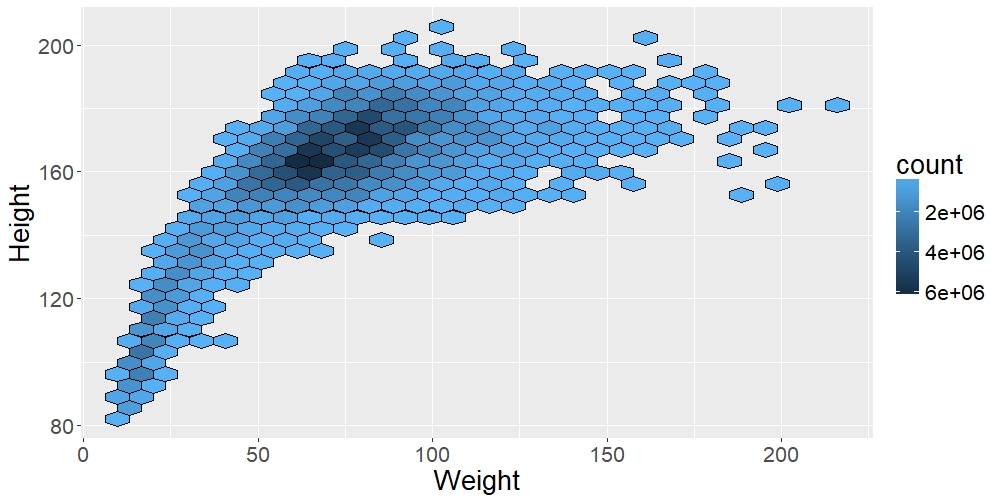
\includegraphics[scale = 0.45]{img/hex-e.jpeg}
\end{center}
\end{frame}
%-------------------------------


%-------------------------------
\begin{frame}{Hexagon Binning}{Method}
\begin{figure}[H]
\centering
    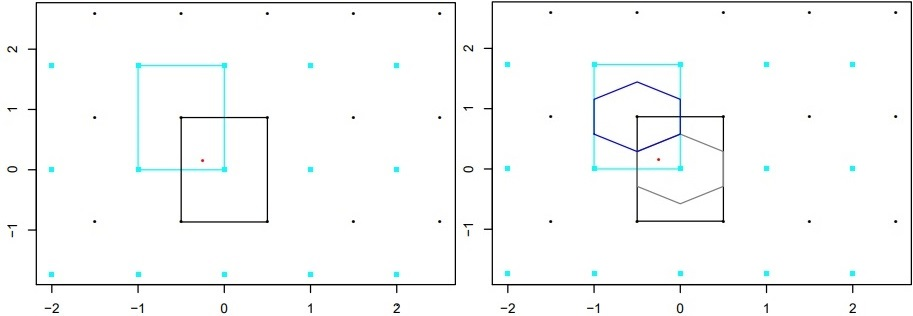
\includegraphics[scale = 0.45]{img/hex-e13.jpg}
    \caption{Hexagon binning explanation, \citep{hexbinfig}}
    \label{fig:hex-e1}
\end{figure}
\end{frame}
%-------------------------------



%[scale = 0.6]
%-------------------------------
\begin{frame}{Times}
\pause
\begin{center}
    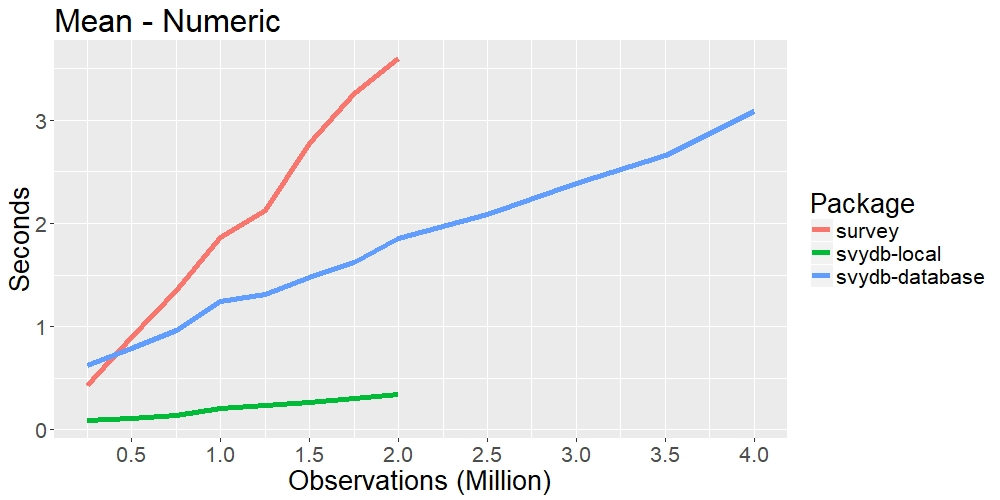
\includegraphics[scale = 0.45]{img/meannum-r.jpeg}
\end{center}
\end{frame}
%-------------------------------



%-------------------------------
\begin{frame}{Times}
\begin{center}
    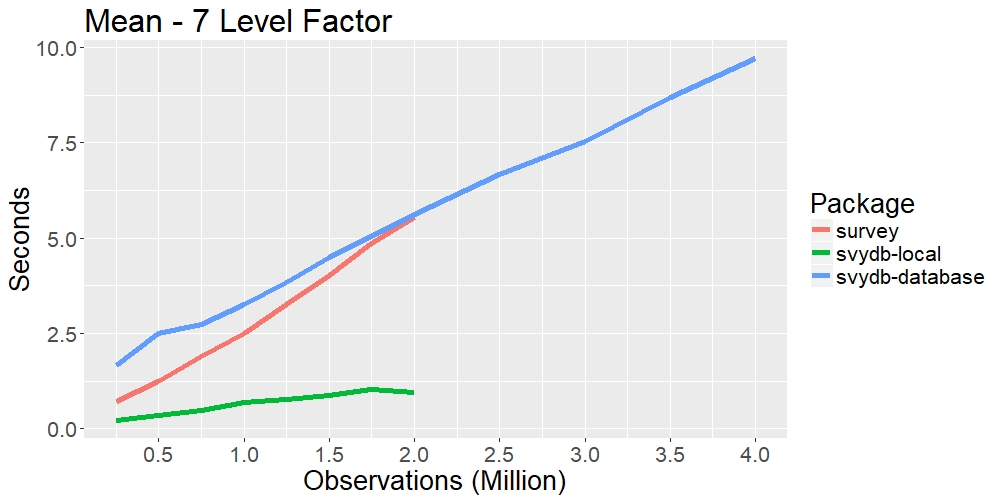
\includegraphics[scale = 0.45]{img/meancat-r.jpeg}
\end{center}
\end{frame}
%-------------------------------


%-------------------------------
\begin{frame}{Times}
\begin{center}
    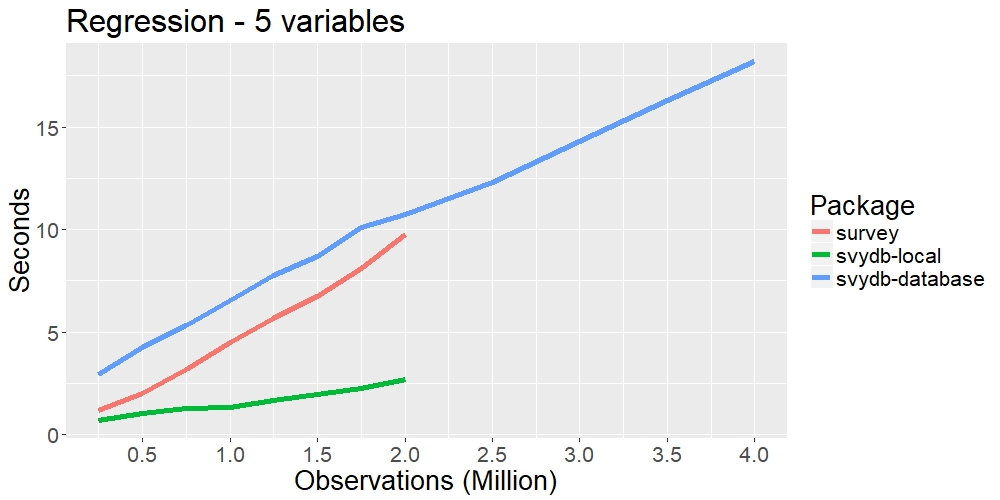
\includegraphics[scale = 0.45]{img/lm-r.jpeg}
\end{center}
\end{frame}
%-------------------------------



%-------------------------------
\begin{frame}{Times}
\begin{center}
    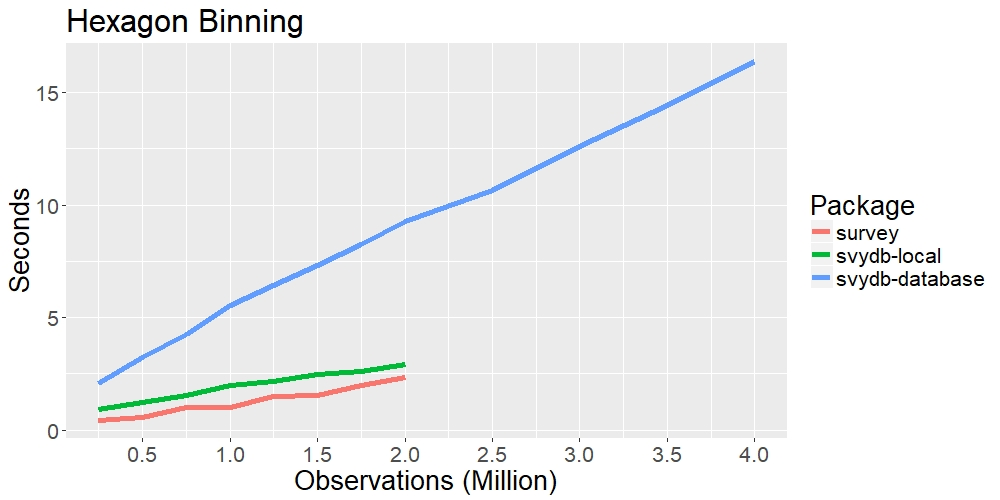
\includegraphics[scale = 0.45]{img/hex-r.jpeg}
\end{center}
\end{frame}
%-------------------------------

%-------------------------------
\begin{frame}[t]{List of functions in svydb}
\begin{columns}[t]
    \begin{column}{0.48\textwidth}
        \begin{itemize}
            \item{Statistics:\\
                \begin{itemize}
                    {\ttfamily
                        \item svydbdesign()
                        \item svydbtotal()
                        \begin{itemize}
                            \item coef()
                            \item SE()
                        \end{itemize}
                        \item svydbmean()
                        \item svydblm()
                        \begin{itemize}
                            \item summary()
                            \item predict()
                        \end{itemize}
                        \item svydbquantile()
                        \item svydbtable()
                        \item svydbby()
                        \item svydbrepdesign()
                        \item svydbreptotal()
                        \item svydbrepmean()
                    }
                \end{itemize}
            }
        \end{itemize}
    \end{column}
    \begin{column}{0.48\textwidth}
        \begin{itemize}
            \item{Graphics\\
                \begin{itemize}
                    {\ttfamily
                        \item svydbhist()
                        \item svydbboxplot()
                        \item svydbhexbin()
                        \item svydbhexplot()
                        \item svydbcoplot()
                    }
                \end{itemize}
            }
        \end{itemize}
    \end{column}
\end{columns}
\end{frame}
%-------------------------------


%-------------------------------
\begin{frame}{Conclusion}
  \begin{itemize}
  \item {
    It is feasible to compute survey statistics in {\sf SQL} as long as:
      \begin{itemize}
          \item {
            No heavy iterations.
          }
          \item {
            Not dependent on mathematical or statistical operations.
          }
      \end{itemize}
  }
  
  \pause
  
  \item{
    Faster on large data sets, for most statistics.
  }
  \pause
  
 \item{
    It can give accurate results, checked with the {\bf survey} package.
 }

  \end{itemize}
\end{frame}
%-------------------------------

\begin{frame}
\begin{center}
    \Huge{Thank You.}
    \nocite{*}
\end{center}
\end{frame}
%-------------------------------

%-------------------------------
{\setbeamerfont{frametitle}{size=\tiny}
    \begin{frame}
    %\bibliography{ref.bib}
    \AtNextBibliography{\tiny}
        \printbibliography
    \end{frame}
}

%-------------------------------

\end{document}


